\documentclass[10pt]{article}

\usepackage{ifthen}
\usepackage{geometry}
\usepackage[usenames,dvipsnames]{color}
\usepackage{marvosym}
\usepackage{wasysym}
\usepackage{enumitem}
\usepackage{setspace}
\usepackage{url}
\usepackage{multicol}
\usepackage{paracol}
\usepackage{fontspec}
\usepackage{xeCJK}
\usepackage{changepage}
\usepackage{listings}
\usepackage{graphicx}

\thispagestyle{empty}\pagestyle{empty}

\XeTeXlinebreaklocale "zh"
% \setCJKmainfont{Source Han Serif SC}

\input{cv.tex}

\begin{document}

\cvtitle{\textbf{Yang Ruini}}{BrickRed}{}{0.5cm}

\positionedbox{left}{0.7\textwidth}{%
Mail: \url{yangruinii@163.com}\\
Github: \url{https://github.com/KKKirino}
}

\begin{picture}(0, 0)
	\put(455, -10){\hbox{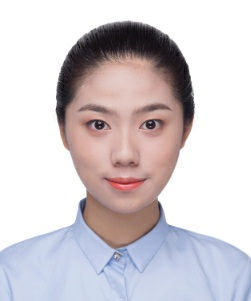
\includegraphics[scale=0.4]{./avatar.png}}}
\end{picture}

\positionedbox{right}{0.3\textwidth}{
	% \begin{picture}(50,50)
	% 	\put(480,0){\hbox{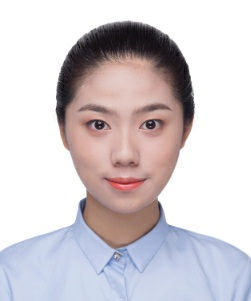
\includegraphics[scale=0.3]{./avatar.png}}}
	% \end{picture}
}

\vspace{0.7cm}

\cvsectiontitle{\textbf{Education}}
\cvcompany{B.Eng. UESTC}{2018.09 - 2022.06}\\
Computer Science, Dept. of Computer Science and Engineering\\

\vspace{.1cm}

GPA: 3.99 / 4.00,CET-4 601,CET-6 553 \\
\textbf{Mathematics and Physics Course Grades:}Mathematical analysis 87、Random Mathematics and Probability Theory 93、Linear algebra 91、Discrete Mathematics 98 \\
\textbf{Computer Professional Course Grades:}Data Structures and Algorithms 85、Operating System 91、Computer Network 87、Artificial Intelligence 99

\vspace{0.8cm}

\cvsectiontitle{\textbf{Projects \& Skills}}
\vspace{-1cm}
\begin{itemize}[leftmargin=0.5cm]
	\item \cvcompany{Sketch Simplification Rendering Based on Reinforcement Learning}{2020.09 - 2021.3}\cvsublevel{%
		\cvsubbullet{%
		Reduce the image dimension through encoder. Simplify the artist's sketch through reinforcement learning framework. A clean sketch directly used for coloring will finally generated. This work refers to a series of sketch simplification work of Waseda University.%
		}%
		\cvsubbullet{%
		Use Pytorch to optimize based on CartoonGAN, AdaIN and U-Net models.
		}
	}

	\item \cvcompany{Flutter-Based Message Application}{2020.12}\cvsublevel{%
		\cvsubbullet{%
		Implement a simple interface UI similar to QQ with Google Flutter framework, and going to implement the message module with Leancloud's message API service and Agora's audio and video API service.%
		}%
	}

	\item \cvcompany{Artificial Intelligence Course Assignment}{2020.09 - 2020.11}\cvsublevel{%
		\cvsubbullet{
			\url{https://github.com/KKKirino/Coding-Every-Day/tree/master/2020/ai-course-exercise}
		}
		\cvsubbullet{%
		Implemente the A* heuristic search algorithm to solve the eight-digit problem. Implement the decision tree establishment and pruning process. Implement the back propagation algorithm of the neural network containing a hidden layer and Sigmoid activation function.%
		}%
		\cvsubbullet{%
		Implemented by Python. Strictly abide by the PEP8 code style specification. Use Python 3 Typing system to improve code readability. Provide complete comments for functions, and ensure code quality.
		}
	}

	\item \cvcompany{Summer Production Internship: National Flight Big Data Visualization Platform}{2020.06 - 2020.08}\cvsublevel{%
		\cvsubbullet{%
		Summer production internship project in the second semester of the sophomore year. Crawl the national flight data based on the Flask + Spark framework. Analyze data by Spark framework. Save the data in the MySQL database. Display it through the front-end page.%
		}%
		\cvsubbullet{%
		Responsible for the front-end page display part. Load the data to the front-end interface through Ajax requests. Use the ECharts chart library for visualization.
		}
	}
\end{itemize}

\vspace{0.4cm}
\cvsectiontitle{\textbf{Honors}}
\vspace{-0.8cm}
\begin{adjustwidth}{0.05cm}{0cm}
	\cvcompany{\small{Google HashCode 2021,International Ranking \#1736(Top 15\%),China Ranking \#32}}{2021.02}\\%
	\cvcompany{\small{Asia and Pacific Mathematical Contest in Modeling 2020 Seocnd Prize}}{2020.11}\\%
	\cvcompany{\small{Second prize Scholarship of Yingcai Honors College of UESTC for two consecutive years}}{2019, 2020}\\%
\end{adjustwidth}
\end{document}